

\begin{wrapfigure}[2]{r}[-1cm]{4cm}
 \vspace{-6cm}
  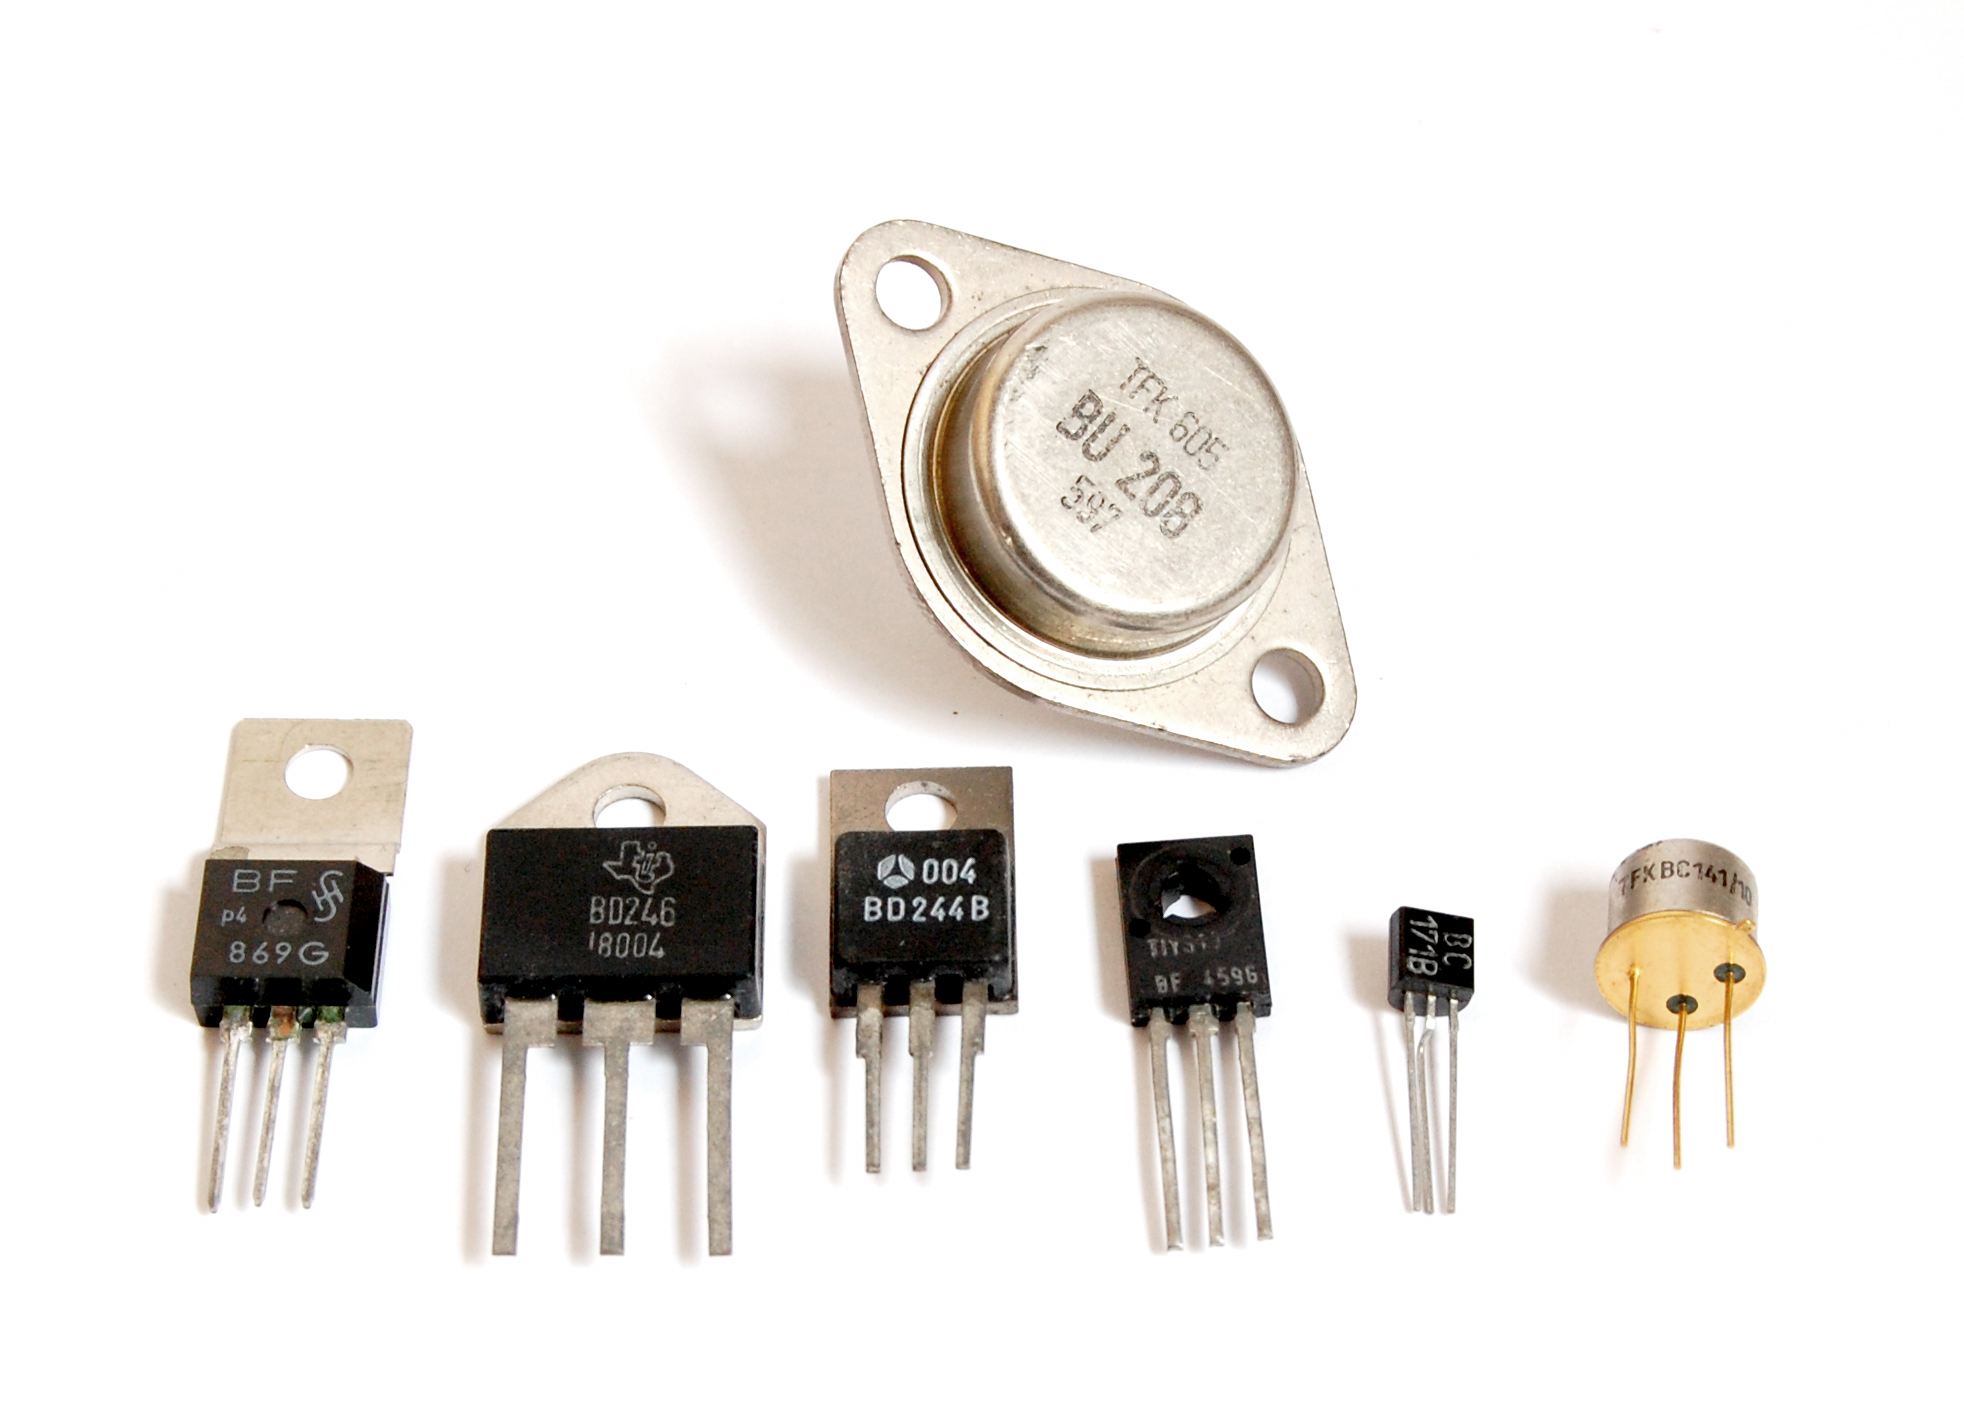
\includegraphics[scale=0.4]{Transistor/Bilder/Transistors-white.jpg}
 \vspace{-6cm}
\end{wrapfigure}

\section{Theorie- und Prüfungsfragen}

~~~~~~

\begin{enumerate}
\itemsep1pt\parskip0pt\parsep0pt
\item[1] Skizziere die Schaltzeichen eines NPN- und eines PNP-Transistors. Beschrifte  entsprechend die Anschlüsse.
\item[2] Zeichne das Ersatzschaltbild aus zwei Dioden für den NPN- und den PNP-Transistor.
\end{enumerate}

\begin{enumerate} 
\itemsep1pt\parskip0pt\parsep0pt
\item[3] \emph{\textbf{TC605}} Welche Kollektorspannungen haben NPN- und PNP-Transistoren?
	\begin{enumerate}
	\itemsep1pt\parskip0pt\parsep0pt
		\item[a] NPN- und PNP-Transistoren benötigen negative Kollektorspannungen.
		\item[b] PNP-Transistoren benötigen positive, NPN-Transistoren negative Kollektorspannung.
		\item[c] PNP- und NPN-Transistoren benötigen positive Kollektorspannungen.
		\item[d] NPN-Transistoren benötigen positive, PNP-Transistoren negative Kollektorspannungen.
	\end{enumerate}
\end{enumerate}



\begin{enumerate} 
\item[4] \emph{\textbf{TC602}}  Das Verhältnis von Kollektorstrom zum Basisstrom eines Transistors liegt üblicherweise im Bereich von
	\begin{enumerate}
	\itemsep1pt\parskip0pt\parsep0pt
		\item[a] 1 zu 50 bis 1 zu 100.
		\item[b] 10 zu 1 bis 900 zu 1.
		\item[c] 1000 zu 1 bis 5000 zu 1.
		\item[d] 1 zu 100 bis 1 zu 500.
	\end{enumerate}
\end{enumerate}

\loesung{

\begin{figure}
\centering
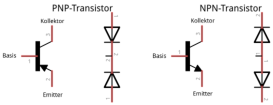
\includegraphics[scale=3]{Transistor/Bilder/PNP_NPN.pdf}
\caption{1 und 2 - NPN- und PNP-Transistor}
\end{figure}

\begin{enumerate}
\itemsep1pt\parskip0pt\parsep0pt
\item[3] d
\item[4] b
\end{enumerate}
}

\section{Praktische Anwendung}

\subsection[Der Bipolar-Transistor als Schalter]{Transistorschaltung 01 - Der Bipolar-Transistor als Schalter}

\begin{itemize}
\itemsep1pt\parskip0pt\parsep0pt
\item Schaue dir den Bipolar-Transistor als Bauteil an und ordne die Bezeichnungen Kollektor, Basis und Emitter den einzelnen Beinchen zu.
\item Baue folgende Transistor-Schaltung auf (Abbildung \ref{s01}). 
\item Lege die Versorgungsspannung an die Schaltung an.
\item Entferne unter Last die Leuchtdiode 1. Welche Auswirkungen hat das auf die Schaltung und warum?
\end{itemize}

\begin{figure}[H]
	\centering
	\subfigure[Schaltplan]{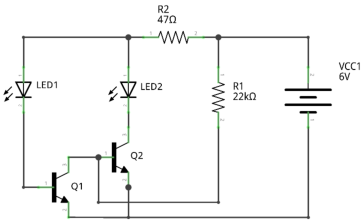
\includegraphics[scale=1.4]{Transistor/Schaltungen/NotBeleuchtung_Schaltplan.pdf}}
	\subfigure[Mögliche Breadboard-Ansicht]{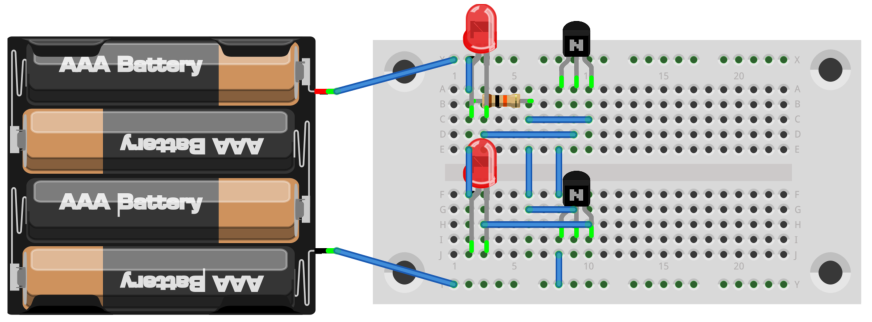
\includegraphics[scale=1]{Transistor/Schaltungen/NotBeleuchtung_Steckplatine.pdf}}
	\caption{Transistorschaltung 01 - Der Bipolar-Transistor als Schalter}
	\label{s01}
\end{figure}

%----------------------------------------------

\subsection[Der Bipolar-Transistor als Sensor]{Transistorschaltung 02 - Der Bipolar-Transistor als Sensor}

\begin{itemize}
\itemsep1pt\parskip0pt\parsep0pt
\item Baue folgende Transistor-Schaltung auf (Abbildung \ref{s02}). 
\item Lege die Versorgungsspannung an die Schaltung an.
\item Berühre die Basis des Transistors Q1 mit dem Finger. Was passiert und warum?
\item \textbf{Zusatz:} Ersetze die Led durch einen Lautsprecher? Was passiert und warum?
\end{itemize}

\begin{figure}[H]
	\centering
	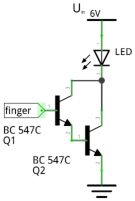
\includegraphics[scale=1.6]{Transistor/Schaltungen/NPN_Sensor.pdf}
	\caption{Transistorschaltung 02 - Der Bipolar-Transistor als Sensor}
	\label{s02}
\end{figure}

%----------------------------------------------

\subsection[Der Bipolar-Transistor als Verstärker]{Transistorschaltung 03 - Der Bipolar-Transistor als Verstärker}

\begin{itemize}
\itemsep1pt\parskip0pt\parsep0pt
\item Baue folgende Transistor-Schaltung auf (Abbildung \ref{s03}). 
\item Lege die Versorgungsspannung an die Schaltung an.
\item Lege ein Audiosignal an den Eingang der Schaltung an. Was passiert und warum?
\end{itemize}

\begin{figure}[H]
	\centering
	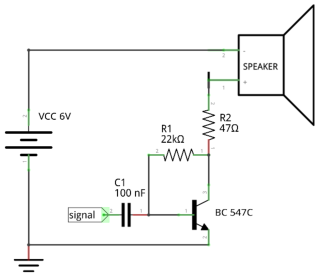
\includegraphics[scale=1.6]{Transistor/Schaltungen/NPN_Verstaerker.pdf}
	\caption{Transistorschaltung 03 - Der Bipolar-Transistor als Sensor}
	\label{s03}
\end{figure}